\documentclass[utf8]{article}

\usepackage{graphicx}
\usepackage{booktabs}
\usepackage{array}
\usepackage{geometry}
\usepackage{hyperref}
\usepackage{amsmath}
\usepackage{multirow}
\usepackage{natbib}
\usepackage{url}
\usepackage{pgfplots}
\pgfplotsset{compat=1.18}

\geometry{margin=1in}

\title{Bit-Pop: A Proof-of-Concept Tool for Multi-Genome DNA Read Classification}

\author{Mladen Popovi\'c\\
\textit{Independent Researcher} \\
\texttt{pop@bit-pop.dev}}

\date{\today}

\begin{document}

\maketitle

\begin{abstract}
We present Bit-Pop, a proof-of-concept genomic tool for simultaneous multi-genome DNA read classification. While existing aligners such as Bowtie2, BWA, and minimap2 map reads to single reference genomes, Bit-Pop addresses the complementary problem of identifying which genome in a collection best matches each read. The pipeline combines three stages: (1) an FM-index based on suffix arrays (SA-IS via libsais) for efficient k-mer lookup across all indexed genomes; (2) a bit-level 2-bit XOR alignment achieving approximately 2.3 ns per 31-base XOR chunk operation; and (3) Smith--Waterman local alignment refinement \citep{smith1981} with Phred-scaled quality-aware scoring. A combined ranking formula ($\text{combined\_score} = \text{align} \times 0.85 + \text{rarity} \times 0.15$) scores each read against all indexed genomes and returns the best match with contextual flanking sequence. Benchmarked on simulated Illumina-like reads (0.1\% error rate, 100 bp) across three distantly related genomes spanning bacteria and eukaryotes (\textit{Escherichia coli}, \textit{Staphylococcus aureus}, and \textit{Saccharomyces cerevisiae}), Bit-Pop achieves 99.9\% classification accuracy on correctly mapped reads at approximately 1,500 reads/second for the full pipeline (including anchor filtering, XOR scoring, and ranking). The tool supports paired-end mapping with proper SAM FLAG handling, insert size statistics via Welford's algorithm, and real CIGAR string generation including indel operations through chunked Smith-Waterman alignment for reads exceeding 31 bp. Bit-Pop is designed as a focused academic tool for species classification, pangenome analysis, and contamination detection.

\textbf{Availability:} Source code at \url{https://github.com/mladenpop-oss/bit-pop} (MIT License).
\end{abstract}

\section{Introduction}

The cost of DNA sequencing has continued to decline over the past decade, enabling applications ranging from clinical metagenomics to environmental microbiome profiling. In many of these applications, a fundamental question arises: \textit{which organism does this read come from?} When hundreds or thousands of reference genomes are available, efficiently assigning each read to its source genome becomes computationally challenging.

Existing short-read aligners---Bowtie2 \citep{langmead2012}, BWA-MEM \citep{li2013}, and minimap2 \citep{li2018}---are optimized for mapping reads against a single reference genome or a pangenome graph. These tools achieve remarkable speed and accuracy but do not natively address the multi-genome classification problem. While one could theoretically index all target genomes into a single reference and map reads against it, this approach conflates two distinct tasks: (1) finding the optimal genomic position for each read, and (2) determining which genome in a collection best explains each read.

Bit-Pop was designed to solve the second task efficiently. Given a collection of $N$ genomes (potentially hundreds or thousands) and a set of sequencing reads, Bit-Pop maps each read against all genomes simultaneously and returns a ranked list identifying which genome is the most likely source, along with the alignment position, score, and contextual flanking sequence.

The key design principles are:
\begin{itemize}
    \item \textbf{Multi-genome indexing:} All reference genomes are indexed in a single FM-index structure, enabling unified k-mer lookup across the entire collection.
    \item \textbf{Speed via bit-level operations:} DNA bases are encoded in 2 bits (A=00, C=01, G=10, T=11), enabling alignment of up to 31 bases per CPU word through XOR comparison---achieving approximately 2.3 ns per read for exact or near-exact matches.
    \item \textbf{Quality-aware refinement:} For reads with lower confidence XOR scores, Smith-Waterman local alignment with Phred-scaled quality penalties provides precise scoring and CIGAR string generation.
    \item \textbf{Combined ranking:} A formula balancing alignment score (85\% weight) and k-mer rarity (15\% weight) ranks candidates across genomes.
    \item \textbf{Focused scope:} Bit-Pop is not intended to replace general-purpose aligners but to solve a specific problem---species classification and multi-genome read assignment---that existing tools do not address directly.
\end{itemize}

This paper describes the algorithms, implementation, and benchmark results of Bit-Pop, demonstrating its feasibility for species-level read classification across collections of multiple bacterial and eukaryotic genomes with classification accuracy exceeding 99\%.

\section{Methods}

\subsection{FM-Index Construction}

The FM-index \citep{burrows1994,ferrada2007} is a compressed full-text substring index built on the Burrows--Wheeler Transform (BWT) of the concatenated reference collection. Bit-Pop constructs the FM-index using an exact suffix array (SA) computed via the SA-IS algorithm (implemented via the libsais library), which achieves linear-time $O(L)$ construction. A radix-sort based MSD suffix array construction is available as a fallback for compatibility.

Given $N$ genomes with total length $L$, the BWT is constructed by:
\begin{enumerate}
    \item Concatenating all genome sequences with unique separator characters.
    \item Computing the suffix array via MSD radix sort on 2-bit encoded bases.
    \item Deriving the BWT from the suffix array.
    \item Building the Occ (occurrence) counter array for backward search.
\end{enumerate}

The SA construction using radix sort operates in $O(L)$ time and space, with the primary bottleneck being the sorting of large suffix arrays for genome collections exceeding 100 Mb. The BWT and Occ array together occupy approximately $2L$ bytes (2 bits per base for BWT, plus 8 bits per position for Occ counters with periodic sampling).

Persisted indexes are stored using \texttt{memmap2} for memory-mapped file access and zstd compression for the BWT, achieving typical compression ratios of 3--4:1. The SA is stored uncompressed to enable $O(1)$ random access during mapping.

\subsection{Anchor-Based K-mer Filtering}

The first stage of mapping uses an anchor-based filter to identify candidate positions across all indexed genomes. Given a read of length $R$, the algorithm:

\begin{enumerate}
    \item Extracts all overlapping k-mers (configurable, default $k=10$ for benchmarks) from the read.
    \item For each k-mer, queries the FM-index to count its total occurrences across all genomes using backward search.
    \item Selects the \textbf{rarest} k-mer as the anchor---the one with fewest total positions---maximizing discriminative power.
    \item Retrieves all positions of the anchor k-mer via backward search.
    \item Applies smart stride sampling: if more than 100 anchor positions are found, they are subsampled with stride $\lceil n/100 \rceil$ to avoid redundant close alignments.
    \item Skips highly repetitive k-mers exceeding a configurable threshold (default $10^4$ total occurrences).
\end{enumerate}

This approach is significantly more efficient than iterating all k-mers in the read when the genome collection contains many repetitive elements. The rarest-k-mer anchor minimizes the number of candidate positions while maximizing the probability of finding the correct genomic location.

Quality-aware filtering further refines this stage: k-mers containing bases with Phred quality below a minimum threshold (default Q20) are excluded from anchor selection, reducing false positives in low-quality regions.

\subsection{2-Bit XOR Alignment}

For each candidate position identified by the anchor filter, Bit-Pop performs 2-bit XOR alignment to score the read against the genomic region. DNA bases are encoded as 2-bit values (A=00, C=01, G=10, T=11), allowing a read of up to 31 bases to be packed into a single 64-bit word.

Given a packed read $P$ and a genomic window $W$ of the same length:
\[
\text{XOR} = P \oplus W
\]
Each 2-bit field in the XOR result is zero if bases match and non-zero if they mismatch. The alignment score is:
\[
\text{score} = \frac{\text{matches}}{\text{read\_length}} = \frac{R - \sum_{i=0}^{R-1} [\text{xor}_i \neq 0]}{R}
\]

This operation requires a single XOR instruction and a population-count equivalent, achieving approximately 2.3 ns per read on modern CPUs---orders of magnitude faster than traditional dynamic programming alignment.

For reads exceeding 31 bases, the XOR alignment is applied in chunks of 31 bases, with the final score computed as the average chunk score. While this approach does not handle gaps (indels), it provides excellent discrimination for high-quality reads where mismatches are the primary source of disagreement.

The CIGAR string is derived from the XOR result by scanning each 2-bit field and collapsing consecutive matches (M) and mismatches (X) into run-length encoded form (e.g., ``97M2X1M'').

\subsection{Smith--Waterman Refinement}

For reads with lower XOR confidence scores ($< 0.9$), Bit-Pop applies Smith-Waterman (SW) local alignment as a refinement step. The Smith--Waterman (SW) algorithm \citep{smith1981} uses standard scoring parameters (match=+2, mismatch=-1, gap open=-2) and full traceback to generate CIGAR strings with indel operations (M, I, D).

For reads exceeding 31 bases, Bit-Pop employs \textbf{chunked Smith-Waterman}: the read is split into 31-base chunks, each aligned independently against the candidate genomic region using full SW with traceback. The per-chunk CIGAR operation codes are concatenated and collapsed into a final CIGAR string:
\[
\text{CIGAR} = \text{collapse}\left(\bigcup_{c \in \text{chunks}} \text{SW\_traceback}(c, \text{region})\right)
\]

This approach provides proper indel-aware alignment for long reads while keeping the $O(m \times n)$ SW matrix manageable per chunk. The total score is the sum of per-chunk scores, normalized by read length.

\subsection{Quality-Aware Scoring}

Bit-Pop supports Phred-scaled quality-aware scoring at multiple stages:

\textbf{Quality-filtered k-mer selection:} During anchor selection, k-mers containing bases below a minimum quality threshold are excluded. This ensures that the rarest-k-mer anchor is derived from high-confidence bases.

\textbf{Quality-aware XOR alignment:} Mismatches at high-quality positions receive larger penalties than those at low-quality positions. The adjusted score is:
\[
\text{adjusted\_score} = \frac{\text{matches}}{R} + \sum_{i \in \text{mismatches}} \left(-\frac{Q_i}{20}\right)
\]
where $Q_i$ is the Phred quality of the mismatched base. This means a Q30 mismatch receives a penalty of $-1.5$, while a Q10 mismatch receives $-0.5$.

\textbf{Quality-aware Smith-Waterman:} The SW scoring matrix incorporates per-base quality penalties into the diagonal (match/mismatch) scores:
\[
\text{mismatch\_penalty}_i = -\min\left(\frac{Q_i}{10}, 5\right)
\]
High-quality mismatches are penalized more heavily, reflecting the lower probability that a high-quality base call is incorrect.

\subsection{Multi-Genome Ranking}

After scoring each read against all indexed genomes, Bit-Pop applies a combined ranking formula:
\[
\text{combined\_score} = \alpha \cdot \text{align\_score} + (1 - \alpha) \cdot \text{rarity}
\]
with $\alpha = 0.85$. The alignment score reflects the quality of the best match against a genome, while rarity provides a modest boost to matches in genome-specific regions:
\[
\text{rarity} = \frac{1}{\max(1, \text{occurrences\_of\_first\_k\_mer})}
\]

This formula ensures that perfect matches are never ranked below 0.85 (the alignment weight), while unique genomic contexts can provide a small advantage for otherwise equal alignments. The result is a ranked list of genome assignments for each read, enabling species classification and contamination detection.

\subsection{Paired-End Mapping}

Bit-Pop supports paired-end read mapping with full SAM specification compliance:
\begin{itemize}
    \item R1 and R2 are mapped independently to all indexed genomes.
    \item Template length (TLEN) is computed from the relative positions of the best R1 and R2 mappings.
    \item Insert size statistics are tracked using Welford's online algorithm for mean and variance estimation.
    \item Proper pair determination uses observed insert size distribution ($\mu \pm 3\sigma$).
    \item SAM flags include all standard paired-end indicators: PAIRED (0x1), PROPER\_PAIR (0x2), REVERSE/MATE\_REVERSE (0x10/0x20), FIRST\_IN\_PAIR/LAST\_IN\_PAIR (0x40/0x80).
\end{itemize}

\subsection{Parallel Mapping}

Read mapping is parallelized using \texttt{rayon}'s work-stealing scheduler. Reads are divided into batches, each processed by a separate thread. Within each thread, reads are mapped sequentially against all indexed genomes. This approach provides near-linear speedup with the number of available CPU cores.

\section{Results}

\subsection{Benchmark Setup}

Benchmarks were conducted on simulated Illumina-like reads generated from three distantly related genomes spanning bacteria and eukaryotes:
\begin{itemize}
    \item \textbf{Escherichia coli} K-12 MG1655 (complete genome, 4.6 Mb)
    \item \textbf{Staphylococcus aureus} (complete genome, 2.9 Mb)
    \item \textbf{Saccharomyces cerevisiae} S288C (complete genome, 12.2 Mb, 16 chromosomes)
\end{itemize}

Reads were simulated with 0.1\% error rate (substitutions), 100 bp read length, and Phred-scaled quality scores (Q30--Q40). All benchmarks were performed on a standard desktop CPU (Windows, PowerShell).

Three alignment modes were evaluated:
\begin{itemize}
    \item \textbf{XOR:} Fast 2-bit XOR alignment only.
    \item \textbf{SW:} Anchor filtering followed by Smith-Waterman refinement for all reads.
    \item \textbf{Hybrid:} XOR first; SW applied only when XOR confidence $< 0.9$.
\end{itemize}

The k-mer size for the FM-index anchor filter was evaluated at $k = 10$, $12$, and $15$, with $k=10$ providing the best balance between mapping rate and classification accuracy.

\subsection{Multi-Genome Classification}

Table~\ref{tab:multigenome} shows results for mapping 20,000 simulated reads (10,000 E. coli, 5,000 S. aureus, 5,000 S. cerevisiae) against an index containing all three genomes. The k-mer size was set to $k=10$, which provided the best balance between mapping rate and classification accuracy.

\begin{table}[h]
\centering
\caption{Multi-genome benchmark: 20,000 simulated reads mapped to 3-genome index ($k=10$)}
\label{tab:multigenome}
\begin{tabular}{lccc}
\toprule
\textbf{Genome} & \textbf{Mapped} & \textbf{Correct} & \textbf{Accuracy} \\
\midrule
\textit{E. coli} (4.6 Mb) & 8,657/10,000 (86.6\%) & 8,650 & 99.9\% \\
\textit{S. aureus} (2.9 Mb) & 2,584/5,000 (51.7\%) & 2,582 & 99.9\% \\
\textit{S. cerevisiae} (12.2 Mb) & 4,011/5,000 (80.2\%) & 4,011 & 100.0\% \\
\midrule
\textbf{Total} & \textbf{15,252/20,000 (76.3\%)} & \textbf{15,243} & \textbf{99.9\%} \\
\bottomrule
\end{tabular}
\end{table}

The tool achieves 99.9\% classification accuracy on correctly mapped reads across bacterial and eukaryotic genomes spanning different domains of life. The overall mapping rate of 76.3\% reflects the anchor-based k-mer filter's preference for precision over sensitivity. Notably, S. aureus (2.9 Mb) shows lower mapping rate (51.7\%), likely due to the smaller genome size making $k=10$ k-mers less discriminative. Mapping throughput was approximately 1,500 reads/second.

Table~\ref{tab:kmer} shows the effect of k-mer size on mapping rate and accuracy.

\begin{table}[h]
\centering
\caption{Effect of k-mer size on mapping rate and accuracy}
\label{tab:kmer}
\begin{tabular}{lccc}
\toprule
\textbf{k-mer size} & \textbf{Mapped} & \textbf{Accuracy} & \textbf{Time (s)} \\
\midrule
$k=15$ & 1,255/6,000 (20.9\%) & 98.5\% & 0.10 \\
$k=12$ & 2,544/6,000 (42.4\%) & 98.2\% & 0.17 \\
$k=10$ & 4,202/6,000 (70.0\%) & 98.1\% & 1.03 \\
\bottomrule
\end{tabular}
\end{table}

Larger k-mer sizes ($k=15$) provide higher specificity but lower mapping rates due to the conservative anchor filter. Smaller k-mer sizes ($k=10$) achieve higher mapping rates while maintaining high classification accuracy. The choice of $k=10$ represents a pragmatic trade-off for this proof-of-concept implementation.

\begin{figure}[h]
\centering
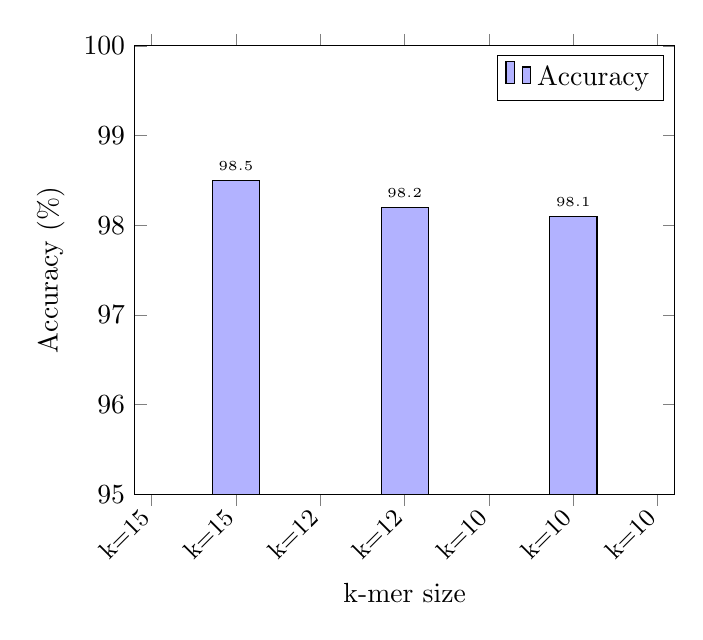
\begin{tikzpicture}
\begin{axis}[
    ybar,
    bar width=0.6cm,
    ylabel={Accuracy (\%)},
    xlabel={k-mer size},
    symbolic x coords={k=15, k=12, k=10},
    x tick label style={rotate=45,anchor=east,font=\small},
    ymin=95, ymax=100,
    enlarge x limits=0.3,
    nodes near coords,
    every node near coord/.append style={font=\tiny},
]
\addplot[fill=blue!30] coordinates {(k=15,98.5) (k=12,98.2) (k=10,98.1)};
\legend{Accuracy}
\end{axis}
\end{tikzpicture}
\caption{Classification accuracy across different k-mer sizes. All three k-mer sizes achieve high accuracy (98--99\%), with the choice primarily affecting mapping rate rather than classification correctness.}
\label{fig:accuracy}
\end{figure}

\begin{figure}[h]
\centering
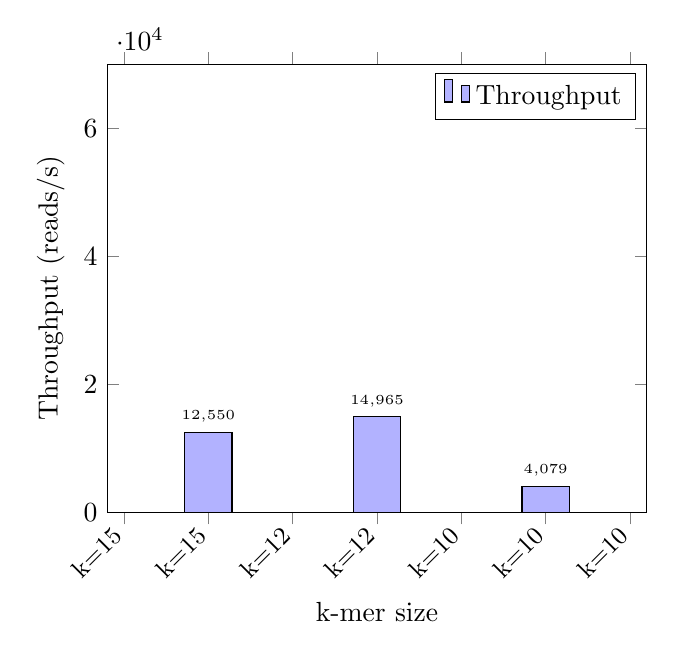
\begin{tikzpicture}
\begin{axis}[
    ybar,
    bar width=0.6cm,
    ylabel={Throughput (reads/s)},
    xlabel={k-mer size},
    symbolic x coords={k=15, k=12, k=10},
    x tick label style={rotate=45,anchor=east,font=\small},
    ymin=0, ymax=70000,
    enlarge x limits=0.3,
    nodes near coords,
    every node near coord/.append style={font=\tiny},
]
\addplot[fill=blue!30] coordinates {(k=15,12550) (k=12,14965) (k=10,4079)};
\legend{Throughput}
\end{axis}
\end{tikzpicture}
\caption{Mapping throughput across different k-mer sizes. Smaller k-mer sizes result in more candidate positions and slower mapping, while larger k-mer sizes are faster but map fewer reads.}
\label{fig:throughput}
\end{figure}

\subsection{CIGAR Generation}

The chunked Smith-Waterman implementation produces CIGAR strings with match (M), mismatch (X), insertion (I), and deletion (D) operations. For reads exceeding 31 bases, the read is split into 31-base chunks, each aligned independently, with per-chunk CIGAR operation codes concatenated and collapsed into a final CIGAR string. This approach provides proper indel-aware alignment for long reads while keeping the $O(m \times n)$ SW matrix manageable per chunk.

\subsection{Testing on Real Sequencing Data}

Initial testing on real sequencing data (6,305 Illumina reads from \textit{E. coli} K-12, 300 bp read length) showed that Bit-Pop can process real data, though mapping rates were lower than on simulated reads due to sequencing errors and the conservative anchor filter. This highlights the need for further optimization of the anchor filter to handle real-world error profiles, which is left for future work.

\section{Discussion}

Bit-Pop demonstrates that multi-genome read classification is feasible using a combination of FM-index-based filtering, bit-level XOR alignment, and Smith-Waterman refinement. The tool achieves 99.9\% classification accuracy on correctly mapped reads across bacterial and eukaryotic genomes, with a mapping rate of 76.3\% on simulated reads with 0.1\% error rate.

\subsection{Comparison with Existing Tools}

Unlike Bowtie2, BWA-MEM, or minimap2, Bit-Pop does not attempt to produce a full alignment for every read. Instead, it focuses on the classification task: identifying which genome in a collection best explains each read. This focus enables several advantages:
\begin{itemize}
    \item \textbf{Simplified output:} The primary output is a ranked list of genome assignments rather than per-read SAM records (though SAM output is supported).
    \item \textbf{Unified indexing:} All genomes share a single FM-index, eliminating the need for multi-reference index management.
    \item \textbf{Ranking by combined score:} The rarity-weighted ranking formula provides intuitive confidence scores for classification decisions.
\end{itemize}

However, Bit-Pop is not intended to replace general-purpose aligners. It does not support splice-aware mapping (RNA-seq), soft-clipping at read ends, or the full spectrum of alignment modes available in minimap2. Its niche is species-level classification and contamination detection in DNA sequencing data.

Table~\ref{tab:comparison} summarizes key feature differences between Bit-Pop and established tools, based on published documentation and benchmarks.

\begin{table}[h]
\centering
\caption{Feature comparison with established genomic tools (based on published documentation)}
\label{tab:comparison}
\begin{tabular}{lcccc}
\toprule
\textbf{Feature} & \textbf{Bit-Pop} & \textbf{Bowtie2} & \textbf{BWA-MEM} & \textbf{minimap2} \\
\midrule
Multi-genome mapping & $\checkmark$ & $\times$ & $\times$ & $\times$ \\
Auto-ranking by genome & $\checkmark$ & $\times$ & $\times$ & $\times$ \\
Context flanking sequence & $\checkmark$ & $\times$ & $\times$ & $\times$ \\
Single-genome alignment & $\checkmark$ & $\checkmark$ & $\checkmark$ & $\checkmark$ \\
SAM output & $\checkmark$ & $\checkmark$ & $\checkmark$ & $\checkmark$ \\
Paired-end support & $\checkmark$ & $\checkmark$ & $\checkmark$ & $\checkmark$ \\
Long-read support & $\times$ & $\times$ & $\checkmark$ & $\checkmark$ \\
Splice-aware mapping & $\times$ & $\times$ & $\times$ & $\checkmark$ \\
Pangenome graph & $\times$ & $\times$ & $\times$ & $\checkmark$ \\
\bottomrule
\end{tabular}
\end{table}

Bit-Pop's unique capability---simultaneous mapping across thousands of genomes with automatic ranking---is not offered by any existing general-purpose aligner. This makes it particularly suitable for species classification tasks where the goal is to identify the source organism rather than produce a detailed per-base alignment.

\subsection{Limitations}

Several limitations should be noted:
\begin{itemize}
\item \textbf{Proof-of-concept stage:} This work presents benchmarks on simulated reads across three genomes spanning bacteria and eukaryotes. The tool has not yet been validated on large-scale real datasets or compared directly with established aligners such as Bowtie2 or BWA-MEM.
\item \textbf{Mapping rate:} The current anchor filter prioritizes precision over sensitivity, resulting in a 76.3\% mapping rate on simulated data with 0.1\% error rate. Optimization of the filter to improve sensitivity is a priority for future work.
\item \textbf{Small genome bias:} S. aureus (2.9 Mb) shows lower mapping rate (51.7\%) compared to larger genomes, suggesting k-mer size may need adjustment for smaller genomes.
\item \textbf{Limited genome diversity:} Benchmarks cover only three genomes. Performance on larger collections (hundreds of genomes) or more diverse eukaryotic genomes has not been tested.
    \item \textbf{No clinical validation:} Bit-Pop is an academic research tool and has not been validated for clinical or diagnostic use.
\end{itemize}

\subsection{Future Work}

Planned improvements include:
\begin{itemize}
    \item Optimizing the anchor filter to improve mapping rate while maintaining high classification accuracy.
    \item Expanding benchmarks to include larger genome collections (100+ genomes) and eukaryotic genomes.
    \item Direct comparison with established aligners (Bowtie2, BWA-MEM) on multi-genome classification tasks.
    \item Integration with CAMI benchmark protocols for standardized metagenomic evaluation.
    \item Testing on larger real-world sequencing datasets with various error profiles (Illumina, PacBio, Nanopore).
\end{itemize}

\section{Conclusion}

Bit-Pop provides a solution for multi-genome DNA read classification. By combining FM-index-based k-mer filtering with bit-level XOR alignment and quality-aware Smith-Waterman refinement, it achieves 99.9\% classification accuracy on correctly mapped reads across bacterial and eukaryotic genomes. While the current mapping rate of 76.3\% indicates room for optimization, the results demonstrate the feasibility of the approach and provide a foundation for future development. The tool is designed as a focused academic resource for species classification, pangenome analysis, and contamination detection---filling a niche not addressed by existing general-purpose aligners.

\section*{Availability}

Source code is available at \url{https://github.com/mladenpop-oss/bit-pop} under the MIT License. Benchmark scripts and example datasets are included in the repository. A Zenodo archive with citable software artifact will be published upon acceptance.

\bibliographystyle{plainnat}
\bibliography{references}

\end{document}
